% !TeX spellcheck = en_US
\newpage
\section{Correlation}
This data science method finds the level of correlation between two data modalities and how predictable they are from each other.

\subsection{Pearson's Correlation}
Given a dataset $(x_i, y_i)^N_{i=1}$ with each instance $i$ having two associated features $x_i$ and $y_i$. Let $\mu_x = \mathbb{E}[x]$ and $\mu_y = \mathbb{E}[y]$ be the dataset \textbf{means} for the two features. The Pearson's correlation is:
\begin{equation}
	\rho = \frac{\overbrace{\mathbb{E}[(x-\mu_x)(y-\mu_y)]}^{\sigma_{xy}}}{\underbrace{\sqrt{\mathbb{E}[(x-\mu_x)^2]}}_{\sigma_x} \cdot \underbrace{\sqrt{\mathbb{E}[(y-\mu_y)^2]}}_{\sigma_y}} \qquad\qquad \rho \in [-1,1]
\end{equation}
A value of $1$ indicates correlation, $-1$ negative correlation and $0$ decorrelation.

\subsubsection{Mutual predictability}
\begin{wrapfigure}[5]{r}{4cm}
	\vspace{-1.5cm}
	\begin{center}
		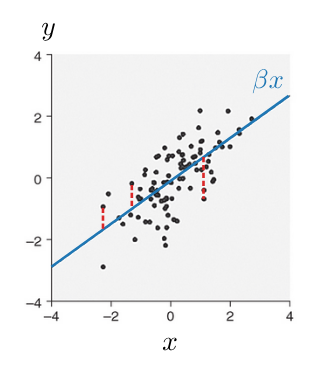
\includegraphics[width=4cm]{pearson}
	\end{center}
\end{wrapfigure}
Lets assume that the data is \textbf{centered}, $\mu_x = \mu_y = 0$, and build a homogeneous linear model that predicts $x$ from $y$ minimizing the square error:
\begin{align*}
	\arg &\min_\beta \mathbb{E}[(y-\beta x)^2]\\
	& = \arg\min_\beta \mathbb{E}[\beta^2x^2 - 2\beta yx]\\
	& = \arg\min_\beta \beta^2\sigma^2_x - 2\beta\sigma_{xy}
\end{align*}
This is a \textbf{convex optimization problem} with solution found at
\begin{equation*}
	\frac{\partial}{\partial\beta}(\beta^2\sigma^2_x - 2\beta\sigma_{xy})=0
\end{equation*}
which gives us the closed form $\beta = \frac{\sigma_{xy}}{\sigma^2_x}$, which injected in the \textit{error function} gives us the error at the optimum, or some measure of predictivity of $y$ from $x$:
\begin{align*}
	\min_\beta & \mathbb{E}[(y - \beta x)^2]\\
	& = \mathbb{E}[(y-\frac{\sigma_{xy}}{\sigma^2_x})^2]\\
	& = \mathbb{E}[y^2] - 2\frac{\sigma_{xy}}{\sigma^2_x} \cdot \mathbb{E}[xy] + \bigg(\frac{\sigma_{xy}}{\sigma^2_x}\bigg)^2 \cdot \mathbb{E}[x^2]\\
	& = \sigma_y ^ 2 - \frac{\sigma_{xy}^2}{\sigma^2_x}\\
	& = \sigma_y ^ 2 \cdot \bigg(1-\bigg(\underbrace{\frac{\sigma_{xy}}{\sigma_x\sigma_y}}_\rho\bigg)^2\bigg)
\end{align*}
Therefore, we have that $\min_\beta \mathbb{E}[(y - \beta x)^2] = \sigma_y^2\cdot (1-\rho^2)$ and $\min_\beta \mathbb{E}[(\beta y - x)^2] = \sigma_x \cdot (1-\rho^2)$, hence there is a \textbf{direct relation} between Pearson's Correlation and mutual predictability

\newpage
\subsection{Canonical Correlation Analysis}
With multivariate data (e.g. images and text, which are composed of multiple features and words) we need to generalize the correlation to modalities of more than one dimension.
\begin{center}
	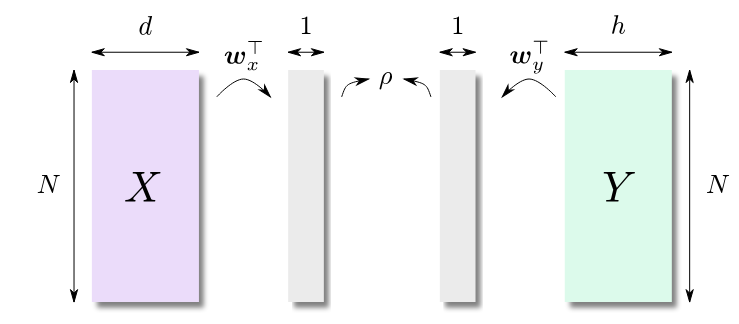
\includegraphics[scale=.3]{cca}
\end{center}
Let $\mathbf{x} \in \mathbb{R}^d$ be the first modality and $\mathbf{y} \in \mathbb{R}^h$ the second one. We want to find the projections $\mathbf{w}_x \in \mathbb{R}^d$ and $\mathbf{w}_y \in \mathbb{R}^h$ of the two modalities in which the Pearson's Correlation is maximized:
\begin{equation*}
	\arg\max_\mathbf{w} \text{Corr}(\mathbf{w}_x^\top \mathbf{x}, \mathbf{w}_y^\top \mathbf{y})
\end{equation*}
\begin{note}
	Since Pearson's Correlation is invariant to the scale of the data, the vectors $\mathbf{w}_x$ and $\mathbf{w}_y$ don't need to be constrained to be e.g. of unit norm.
\end{note}

The correlation can be rewritten as
\begin{align}
	\begin{split}
		\text{Corr}&(\mathbf{w}_x^\top, \mathbf{x}, \mathbf{w}_y^\top \mathbf{y}) \\
		& = \frac{\mathbb{E}[(\mathbf{w}_x^\top(\mathbf{x}-\mathbf{\mu}_x) \cdot  (\mathbf{w}_y^\top(\mathbf{y}-\mathbf{\mu}_y)))]}{\sqrt{\mathbb{E}[(\mathbf{w}_x^\top(\mathbf{x}-\mathbf{\mu}_x))^2]} \cdot \sqrt{\mathbb{E}[(\mathbf{w}_y^\top(\mathbf{y}-\mathbf{\mu}_y))^2]}} \\
		& = \frac{\mathbf{w}_x^\top C_{xy}\mathbf{w}_y}{\sqrt{\mathbf{w}^\top_x C_{xx}\mathbf{w}_x} \cdot \sqrt{\mathbf{w}^\top_y C_{yy}\mathbf{w}_y}} \label{eq:cca}
	\end{split}
\end{align}
where
\begin{align*}
	& C_{xy} = \mathbb{E}[(\mathbf{x}-\mathbf{\mu}_x)(\mathbf{y}-\mathbf{\mu}_y)^\top] \\
	& C_{xx} = \mathbb{E}[(\mathbf{x}-\mathbf{\mu}_x)(\mathbf{x}-\mathbf{\mu}_x)^\top] \\
	& C_{yy} = \mathbb{E}[(\mathbf{y}-\mathbf{\mu}_y)(\mathbf{y}-\mathbf{\mu}_y)^\top]
\end{align*}
are cross-covariance and auto-covariance matrices that can be precomputed. Since the optimum of the problem (as seen in the rewriting of correlation) is specified up to a scaling of $\mathbf{w}_x$ and $\mathbf{w}_y$, we can force a particular scale to get a simpler optimization. In particular we can reformulate it as a \textbf{standard quadratic optimization problem} with quadratic constraints:
\begin{align*}
	\arg \max_\mathbf{w} \mathbf{w}^\top_x C_{xy}\mathbf{w}_y \qquad \text{such that} \qquad & \mathbf{w}_x^\top C_{xx}\mathbf{w}_x = 1 \\
	& \mathbf{w}_y^\top C_{yy}\mathbf{w}_y = 1
\end{align*}
We can then obtain a closed form solution through the Lagrange multipliers method, which is the first eigenvector with highest eigenvalue of the generalized eigenvalue problem:
\begin{equation}
	\begin{bmatrix}
		0 & C_{xy} \\
		C_{yx} & 0
	\end{bmatrix} \begin{bmatrix}
	\mathbf{w}_x \\ \mathbf{w}_y
	\end{bmatrix} = \lambda \begin{bmatrix}
	C_{xx} & 0 \\
	0 & C_{yy} 
	\end{bmatrix} \begin{bmatrix}
	\mathbf{w}_x \\ \mathbf{w}_y
	\end{bmatrix}
\end{equation}
With the eigenvalue $\lambda$ representing the correlation $\rho$ of data in the two projected spaces.
\newpage
\subsubsection{High Dimensions}
CCA generalized problem may be too expensive to solve if $d$ is large because it involves the eigendecomposition of matrices of size $d \times d$. To solve this, we force the solution to be a weighted combination of the data:
\begin{align*}
	& \mathbf{w}_x = \sum_{i=1}^{N} (\mathbf{x}_i-\mu_x)\alpha_{x,i} = \tilde{X}\mathbf{\alpha}_x \qquad\qquad \mathbf{\alpha}_x \in \mathbb{R}^N\\
	& \mathbf{w}_y = \sum_{i=1}^{N} (\mathbf{y}_i-\mu_y)\alpha_{y,i} = \tilde{Y}\mathbf{\alpha}_y \qquad\qquad \mathbf{\alpha}_y \in \mathbb{R}^N
\end{align*}
with $\tilde{X}$ and $\tilde{Y}$ being two matrices containing the \textbf{centered} data. Therefore we have that CCA with $\mathbf{\alpha}$ injected becomes:
\begin{align*}
	\arg \max_\mathbf{\alpha} \overbrace{\mathbf{\alpha}_x^\top\tilde{X}^\top}^{\mathbf{w}_x^\top}C_{xy}\overbrace{\tilde{Y}\mathbf{\alpha}_y}^{\mathbf{w}_y} \qquad \text{such that} \qquad & \overbrace{\mathbf{\alpha}_x^\top\tilde{X}^\top}^{\mathbf{w}_x^\top}C_{xx}\overbrace{\tilde{X}\mathbf{\alpha}_x}^{\mathbf{w}_x} = 1 \\
	& \underbrace{\mathbf{\alpha}_y^\top\tilde{Y}^\top}_{\mathbf{w}_y^\top}C_{yy}\underbrace{\tilde{Y}\mathbf{\alpha}_y}_{\mathbf{w}_y} = 1
\end{align*}
Observing that:
\begin{itemize}
	\item $C_{xy} = \frac{1}{N}\tilde{X}\tilde{Y}^\top$
	\item $C_{xx} = \frac{1}{N}\tilde{X}\tilde{X}^\top$
	\item $C_{yy} = \frac{1}{N}\tilde{Y}\tilde{Y}^\top$
\end{itemize}
the objective becomes
\begin{align*}
	\arg\max_\mathbf{\alpha} \mathbf{\alpha}_x^\top \overbrace{\frac{1}{N}\tilde{X}^\top\tilde{X}\tilde{Y}^\top\tilde{Y}}^{Q_{xy}}\mathbf{\alpha}_y \qquad \text{such that} \qquad & \mathbf{\alpha}_x^\top \overbrace{\frac{1}{N}\tilde{X}^\top \tilde{X}\tilde{X}^\top\tilde{X}}^{Q_{xx}} \mathbf{\alpha}_x = 1 \\
	& \mathbf{\alpha}_y^\top \underbrace{\frac{1}{N}\tilde{Y}^\top \tilde{Y}\tilde{Y}^\top\tilde{Y}}_{Q_{yy}} \mathbf{\alpha}_y = 1
\end{align*}
where $Q_{xy}$, $Q_{xx}$ and $Q_{yy}$ are matrices of size $N \times N$ instead of $d \times d$. At this point we have the formulation of the optimization problem that's in the same form as the original CCA but with different matrices and optimization variables
\begin{align}
	\begin{split}
		\arg\max_\mathbf{\alpha} \mathbf{\alpha}_x^\top Q_{xy} \mathbf{\alpha}_y \qquad \text{such that} \qquad & \mathbf{\alpha}_x^\top Q_{xx} \mathbf{\alpha}_x = 1 \\
		& \mathbf{\alpha}_y^\top Q_{yy} \mathbf{\alpha}_y = 1
	\end{split}
\end{align}
and therefore we can use the same framework of Lagrange multipliers to find the solution $\mathbf{\alpha}$ as the leading eigenvector of a generalized eigenvalue problem
\begin{equation}
	\underbrace{
		\begin{bmatrix}
			0 &  Q_{xy} \\
			Q_{yx} & 0
	\end{bmatrix}}_A \begin{bmatrix}
	\mathbf{\alpha}_x \\ \mathbf{\alpha}_y
\end{bmatrix} = \lambda \underbrace{\begin{bmatrix}
	Q_{xx} & 0 \\
	0 & Q_{yy}
	\end{bmatrix}}_{B} \begin{bmatrix}
	\mathbf{\alpha}_x \\ \mathbf{\alpha}_y
\end{bmatrix}
\end{equation}

\begin{note}
	For \textbf{stability} it's useful to add a small diagonal term on the matrix $B$.
\end{note}

\newpage
\subsubsection{Temporal}
If variables are coupled with delays (e.g. medical data from different sources like fMRI and spectrogram of neural activity), simultaneous samples will not be coupled and standard CCA will not find the right solution.\\
The solution is to \textbf{shift} one variable relative to the other and maximize the correlation for a sum over all relative time lags.
\begin{equation}
	\underset{w_x(\tau), w_y}{\text{argmax}} \text{Corr}\bigg(\sum_\tau w_x(\tau)^\top x(t-\tau), w_y^\top y(t)\bigg)
\end{equation}
We can then create $\tilde{X}$ and $\tilde{w}_x$ and obtain:
\begin{equation}
	\underset{w_{\tilde{x}}, w_y}{\text{argmax}} \text{Corr}(\tilde{w}_x^\top \tilde{X}, w_y^\top Y) \qquad\qquad \tilde{X} = \begin{bmatrix}
		X_{\tau_1} \\ X_{\tau_2} \\ \vdots \\ X_{\tau_T}
	\end{bmatrix} \qquad
	\tilde{w}_x = \begin{bmatrix}
		w_x(\tau_1) \\ w_x(\tau_2) \\ \vdots \\ w_x(\tau_T)
	\end{bmatrix}
\end{equation}

\begin{note}
	In case of \textbf{high dimensionality} we can represent $w_x$ as a weighted combination of the data:
	\begin{equation}
		w_x = X\alpha_x
	\end{equation}
\end{note}

\subsection{Nonlinear Correlations}
In situations where we have a negligible (close to $0$) Pearson's Correlation coefficient we can nonlinearly expand $x$ and $y$ and apply CCA to find a correlation in the expanded space.

\begin{example}
	In this case we expand $x$ to $\phi(x)=[x,x^2,x^3]$ and $y$ to $\phi(y)=[y,y^2,y^3]$ and calculate CCA on both of them. The result is:
	\begin{equation*}
		\lambda_1 = 0.86 \qquad\qquad \mathbf{u}_1 = [\underbrace{-0.13, 1.84, 0.15}_{\mathbf{w}_x}, \underbrace{0.09, -1.88, -0.07}_{\mathbf{w}_y}]
	\end{equation*}
	We notice that 
	\begin{equation*}
		\text{Corr}(0+ x^2+0, 0-y^2+0) \approx 0.86
	\end{equation*}
	and that therefore the data is governed by the equation $x^2 = \alpha(-y^2)+\beta$, where setting $\alpha=1$ and $\beta=1$ gives us $x^2+y^2=1$.
	\begin{center}
		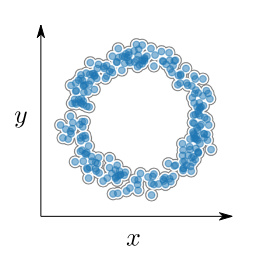
\includegraphics[scale=0.4]{nonlin1}
		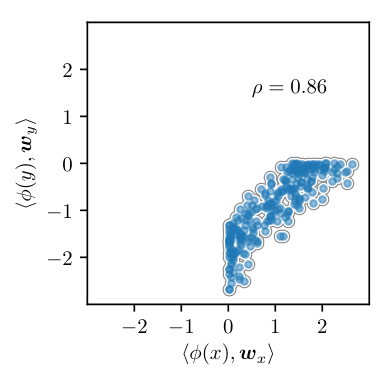
\includegraphics[scale=0.3]{nonlin2}
	\end{center}
\end{example}